\documentclass[14pt]{extbook}
\usepackage{multicol, enumerate, enumitem, hyperref, color, soul, setspace, parskip, fancyhdr} %General Packages
\usepackage{amssymb, amsthm, amsmath, latexsym, units, mathtools} %Math Packages
\everymath{\displaystyle} %All math in Display Style
% Packages with additional options
\usepackage[headsep=0.5cm,headheight=12pt, left=1 in,right= 1 in,top= 1 in,bottom= 1 in]{geometry}
\usepackage[usenames,dvipsnames]{xcolor}
\usepackage{dashrule}  % Package to use the command below to create lines between items
\newcommand{\litem}[1]{\item#1\hspace*{-1cm}\rule{\textwidth}{0.4pt}}
\pagestyle{fancy}
\lhead{Module5}
\chead{}
\rhead{Version C}
\lfoot{3697-2165}
\cfoot{}
\rfoot{test}
\begin{document}

\begin{enumerate}
\litem{
Solve the radical equation below. Then, choose the interval(s) that the solution(s) belongs to.\[ \sqrt{-30 x^2 - 63} - \sqrt{-87 x} = 0 \]\begin{enumerate}[label=\Alph*.]
\item \( x_1 \in [1.17, 1.47] \text{ and } x_2 \in [-0.5,5.5] \)
\item \( x_1 \in [-1.58, -1.2] \text{ and } x_2 \in [-3.5,0.5] \)
\item \( \text{All solutions lead to invalid or complex values in the equation.} \)
\item \( x \in [1.17,1.47] \)
\item \( x \in [1.47,1.5] \)

\end{enumerate} }
\litem{
What is the domain of the function below?\[ f(x) = \sqrt[4]{3 x - 5} \]\begin{enumerate}[label=\Alph*.]
\item \( [a, \infty), \text{where } a \in [-1.47, 0.82] \)
\item \( [a, \infty), \text{ where } a \in [0.98, 2.8] \)
\item \( (-\infty, a], \text{where } a \in [0.67, 6.67] \)
\item \( (-\infty, \infty) \)
\item \( (-\infty, a], \text{where } a \in [0.6, 1.6] \)

\end{enumerate} }
\litem{
Choose the equation of the function graphed below.
\begin{center}
    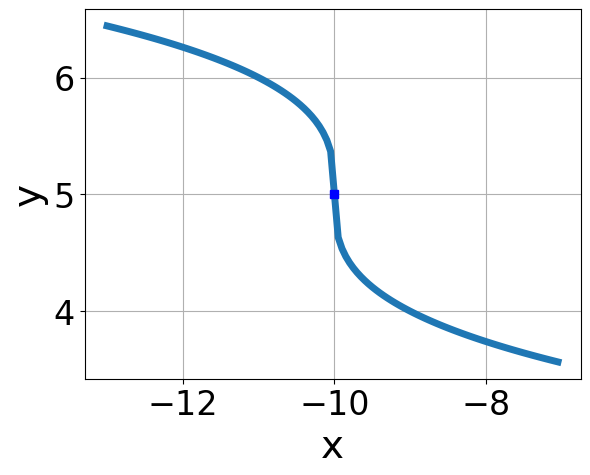
\includegraphics[width=0.5\textwidth]{../Figures/radicalGraphToEquationC.png}
\end{center}
\begin{enumerate}[label=\Alph*.]
\item \( f(x) = \sqrt{x - 6} + 7 \)
\item \( f(x) = \sqrt{x + 6} + 7 \)
\item \( f(x) = - \sqrt{x - 6} + 7 \)
\item \( f(x) = - \sqrt{x + 6} + 7 \)
\item \( \text{None of the above} \)

\end{enumerate} }
\litem{
Solve the radical equation below. Then, choose the interval(s) that the solution(s) belongs to.\[ \sqrt{27 x^2 - 15} - \sqrt{36 x} = 0 \]\begin{enumerate}[label=\Alph*.]
\item \( x \in [1.56,1.86] \)
\item \( x_1 \in [-0.06, 0.56] \text{ and } x_2 \in [-0.33,2.67] \)
\item \( x_1 \in [-0.55, -0.26] \text{ and } x_2 \in [-0.33,2.67] \)
\item \( \text{All solutions lead to invalid or complex values in the equation.} \)
\item \( x \in [-0.55,-0.26] \)

\end{enumerate} }
\litem{
Choose the equation of the function graphed below.
\begin{center}
    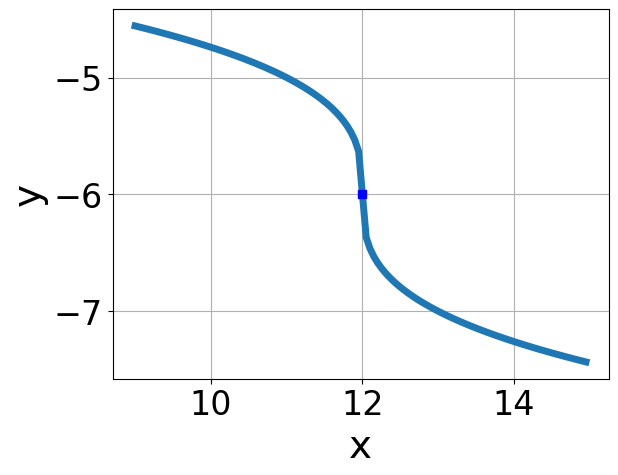
\includegraphics[width=0.5\textwidth]{../Figures/radicalGraphToEquationCopyC.png}
\end{center}
\begin{enumerate}[label=\Alph*.]
\item \( f(x) = \sqrt{x - 10} - 4 \)
\item \( f(x) = \sqrt{x + 10} - 4 \)
\item \( f(x) = - \sqrt{x + 10} - 4 \)
\item \( f(x) = - \sqrt{x - 10} - 4 \)
\item \( \text{None of the above} \)

\end{enumerate} }
\litem{
What is the domain of the function below?\[ f(x) = \sqrt[5]{9 x - 3} \]\begin{enumerate}[label=\Alph*.]
\item \( \text{The domain is } [a, \infty), \text{   where } a \in [0.9, 4.3] \)
\item \( \text{The domain is } (-\infty, a], \text{   where } a \in [0.9, 3.1] \)
\item \( \text{The domain is } (-\infty, a], \text{   where } a \in [0, 1.2] \)
\item \( \text{The domain is } [a, \infty), \text{   where } a \in [-3.5, 0.8] \)
\item \( (-\infty, \infty) \)

\end{enumerate} }
\litem{
Choose the graph of the equation below.\[ f(x) = - \sqrt[3]{x + 10} + 4 \]\begin{enumerate}[label=\Alph*.]
\begin{multicols}{2}\item 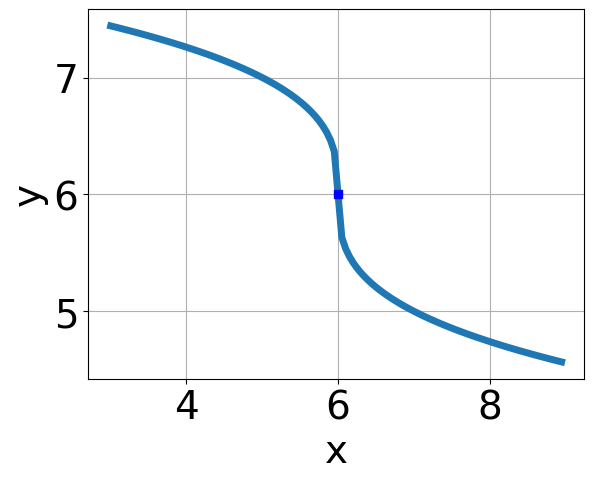
\includegraphics[width = 0.3\textwidth]{../Figures/radicalEquationToGraphAC.png}\item 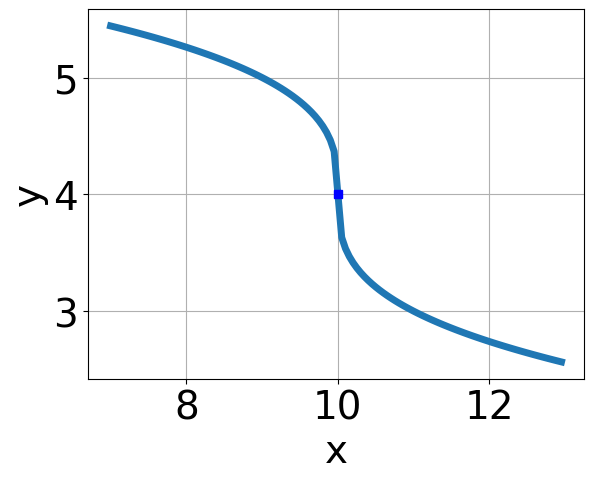
\includegraphics[width = 0.3\textwidth]{../Figures/radicalEquationToGraphBC.png}\item 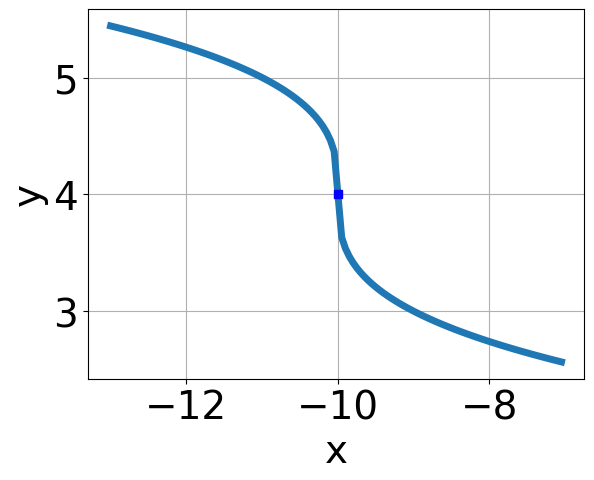
\includegraphics[width = 0.3\textwidth]{../Figures/radicalEquationToGraphCC.png}\item 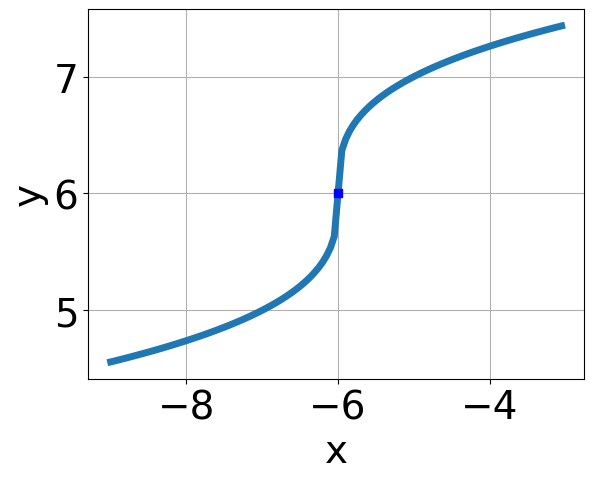
\includegraphics[width = 0.3\textwidth]{../Figures/radicalEquationToGraphDC.png}\end{multicols}\item None of the above.
\end{enumerate} }
\litem{
Solve the radical equation below. Then, choose the interval(s) that the solution(s) belongs to.\[ \sqrt{-8 x + 6} - \sqrt{8 x + 5} = 0 \]\begin{enumerate}[label=\Alph*.]
\item \( x \in [0.36,1.39] \)
\item \( x \in [-0.01,0.16] \)
\item \( x_1 \in [-1.23, -0.47] \text{ and } x_2 \in [0.75,4.75] \)
\item \( \text{All solutions lead to invalid or complex values in the equation.} \)
\item \( x_1 \in [-0.01, 0.16] \text{ and } x_2 \in [0.75,4.75] \)

\end{enumerate} }
\litem{
Choose the graph of the equation below.\[ f(x) = \sqrt[3]{x + 8} + 4 \]\begin{enumerate}[label=\Alph*.]
\begin{multicols}{2}\item 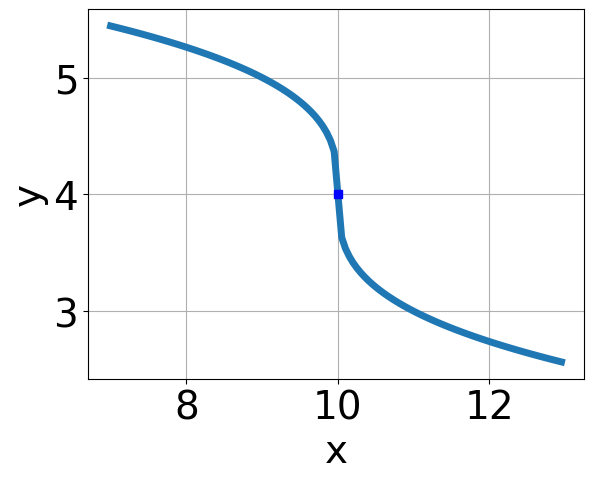
\includegraphics[width = 0.3\textwidth]{../Figures/radicalEquationToGraphCopyAC.png}\item 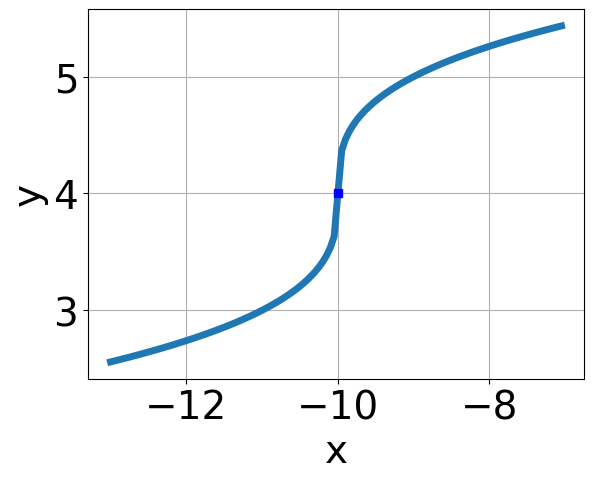
\includegraphics[width = 0.3\textwidth]{../Figures/radicalEquationToGraphCopyBC.png}\item 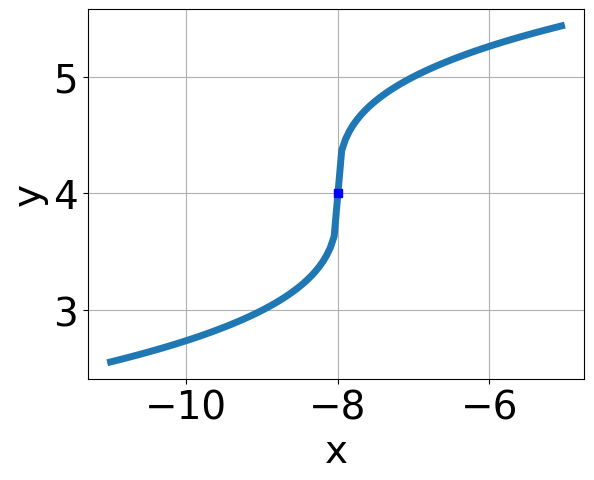
\includegraphics[width = 0.3\textwidth]{../Figures/radicalEquationToGraphCopyCC.png}\item 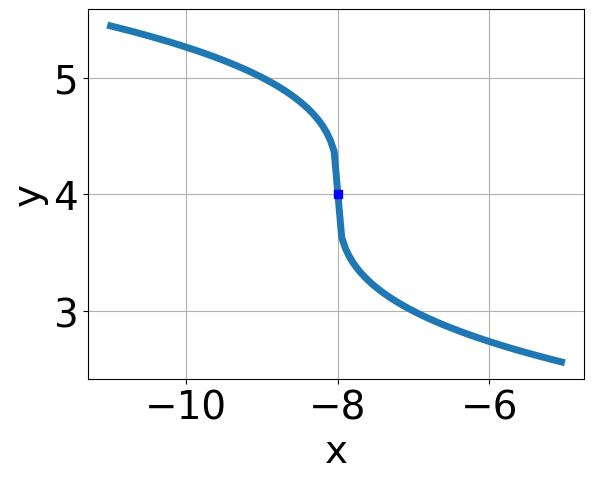
\includegraphics[width = 0.3\textwidth]{../Figures/radicalEquationToGraphCopyDC.png}\end{multicols}\item None of the above.
\end{enumerate} }
\litem{
Solve the radical equation below. Then, choose the interval(s) that the solution(s) belongs to.\[ \sqrt{6 x + 9} - \sqrt{-8 x + 9} = 0 \]\begin{enumerate}[label=\Alph*.]
\item \( x_1 \in [-1.63, -1.4] \text{ and } x_2 \in [0.65,3.2] \)
\item \( \text{All solutions lead to invalid or complex values in the equation.} \)
\item \( x \in [-0.32,0.21] \)
\item \( x \in [-1.3,-1.23] \)
\item \( x_1 \in [-1.63, -1.4] \text{ and } x_2 \in [-0.77,0.54] \)

\end{enumerate} }
\end{enumerate}

\end{document}